\documentclass[11pt]{article}

\usepackage[review]{acl}

\usepackage{times}
\usepackage{latexsym}

\usepackage[T1]{fontenc}
\usepackage[utf8]{inputenc}
\usepackage{microtype}
\usepackage{inconsolata}
\usepackage{graphicx}
\usepackage{amsmath}
\usepackage{amssymb}
\usepackage{amsthm}
\usepackage{booktabs}
\usepackage{colortbl}
\usepackage{multirow}
\usepackage{xcolor}
\usepackage{pifont}
\usepackage{tikz}
\usetikzlibrary{arrows.meta,positioning,calc,fit,backgrounds,decorations.pathreplacing,shadows.blur}

\definecolor{cRef}{HTML}{1F5C99}
\definecolor{cBad}{HTML}{C0392B}
\definecolor{cGood}{HTML}{2E8B57}
\definecolor{cInk}{HTML}{242424}
\definecolor{cMut}{HTML}{7C7C7C}
\definecolor{cGrid}{HTML}{D8DEE6}
\definecolor{cFill}{HTML}{EAF1F8}
\definecolor{cWarn}{HTML}{E67E22}
\tikzset{
  vstep/.style={draw=cGood!70!black, line width=0.5pt, fill=cGood!14, rounded corners=2pt,
                minimum width=0.66cm, minimum height=0.46cm, font=\scriptsize, inner sep=1pt, text=cInk},
  fstep/.style={draw=cBad!75!black, line width=0.5pt, fill=cBad!12, rounded corners=2pt,
                minimum width=0.66cm, minimum height=0.46cm, font=\scriptsize, inner sep=1pt, text=cInk},
  pstep/.style={draw=cBad!55!black, line width=0.5pt, fill=cBad!6, rounded corners=2pt,
                minimum width=0.66cm, minimum height=0.46cm, font=\scriptsize, inner sep=1pt,
                text=cBad!70!black, dash pattern=on 1.6pt off 1.2pt},
  lane/.style={font=\scriptsize\bfseries, text=cInk},
  flow/.style={-{Stealth[length=4pt]}, line width=0.6pt, draw=cMut},
  prop/.style={-{Stealth[length=4pt]}, line width=0.7pt, draw=cBad!80!black, dash pattern=on 2pt off 1.5pt},
  axis/.style={-{Stealth[length=4pt]}, line width=0.6pt, draw=cInk},
  gridln/.style={draw=cGrid, line width=0.4pt},
  tick/.style={font=\scriptsize, text=cMut},
}

\newtheorem{proposition}{Proposition}

\emergencystretch=3em

\title{When Do Errors Compound Across Languages?\\
Heterogeneous Multilingual Reliability of Long-Horizon Agentic Tool Use}

\author{Anonymous ACL submission}

\begin{document}
\maketitle

\begin{abstract}
Tool-calling agents are evaluated almost entirely in English, and the little
multilingual evidence that exists studies single function calls. We ask what
happens over a long horizon. We evaluate frontier backbones on executable BFCL
multi-turn environments whose user queries are localized into eight
typologically diverse languages while the tool interfaces remain
language-invariant, so that success is graded by the post-execution system state
with execution-based grading rather than model-judge annotation. Our central
finding is not a universal compounding story. Instead, the BFCL results show
\emph{heterogeneous}
multilingual long-horizon behavior: some backbone--language cells move
directionally toward compounding relative to an independent-error null, others
are largely explained by weaker single-step validity alone, and the main
comparison is therefore restricted to backbones that provide usable English
baselines. We therefore pair the
compounding-factor analysis with a step-stage decomposition over intent and tool
selection, argument and parameter formatting, and sequencing and planning,
alongside matched-validity detour-conditioned failure and recovery analysis.
This asks not only whether non-English steps are
weaker, but whether non-English trajectories are less able to recover once they
go off reference. Across the main interpretable backbones (Gemini 3 Flash
Preview and Claude Sonnet 4.6), no non-English cell meets the Holm threshold for
$\mathrm{CF}>1$ under the $200$-resample procedure used here; the strongest
directional cell is Turkish on Gemini 3
Flash Preview
($\mathrm{CF}=1.24$ at $K=10$). Descriptively, on shared replay-validity bins,
non-English trajectories end in failure after off-reference detours more often
than English ones ($0.353$ vs.\ $0.143$) and recover less often ($0.647$ vs.\
$0.857$). The dominant failure
mix in the headline cells is intent/selection and sequencing rather than
argument-boundary mismatch, so we do not evaluate the proposed canonicalization
mitigation. All $32/32$ localized BFCL queries pass
reference-call invariance, and the low-fidelity filter removes none of the
evaluated slice. The contribution is therefore a measurement and decomposition
framework: BFCL localizes where multilingual long-horizon reliability degrades,
where it is explained by step-level weakness alone, and where genuine
trajectory-level differences remain. Code repository can be accessed at the following link: \url{https://anonymous.4open.science/r/multilingual-compounding-5A88/}
\end{abstract}

\section{Introduction}
\label{sec:intro}

Large language models are increasingly deployed as agents that complete tasks by
issuing structured function calls to external tools over many turns
\citep{patil2025bfcl,yao2025taubench}. Almost all evaluation of this capability
is conducted in English. The little multilingual evidence that exists is recent
and confined to a \emph{single} function call: \citet{mlcl2026} show that when a
user query is posed in a non-English language, models often produce a
semantically reasonable but non-executable call, a failure they name parameter
value language mismatch (for example, filling a categorical argument with a word
in the user's language where the tool expects a fixed English enumeration value). In parallel, a separate body of work studies
\emph{long-horizon} tool use, where errors accumulate across steps
\citep{denoiseflow2026,phgpo2026,htc2026}, but it is conducted entirely in
English. Neither line answers the question that matters for multilingual
deployment: over a long trajectory, does a small per-step language penalty stay
small, or does it compound?

This question is not answered by composing the two literatures. A per-step
penalty could be benign if errors are independent and recoverable, or severe if a
single early language-induced error derails the remaining steps. The difference is
the whole story for whether agents are usable outside English, and it is invisible
to single-turn evaluation by construction.

We study it directly and with execution ground truth. In this paper we focus on
BFCL v3 multi-turn tasks, whose success is determined by the post-execution
system state \citep{patil2025bfcl}. We localize their user-facing queries into
eight typologically diverse languages and keep the tool schemas
language-invariant in English, which mirrors real deployment where interfaces
are fixed and only the user changes language. Because success is graded by
execution, no human annotator labels task outcomes or tool-call validity; query
translation is a
data-preparation step that we validate by back-translation and a
reference-call invariance check (Section~\ref{sec:experiments}). We analyze
trajectories, not just final calls, and use BFCL as the evidence base for this
study.

Our contributions are as follows.
\begin{enumerate}
\itemsep0.2em
\item \textbf{An execution-grounded BFCL study of multilingual long-horizon
tool reliability that directly tests where
cross-lingual gaps exceed a step-level null.} Prior work treats these pieces
separately: single-turn multilingual tool calling
\citep{mlcl2026,arabicenglish2026}, monolingual long-horizon compounding
\citep{fintoolbench2026}, and monolingual single- versus multi-turn baseline and
propagation measurement \citep{turnwise2026,agentprop2026}. We study their
intersection on execution ground truth, with execution-based scoring rather
than judge labels.
\item \textbf{A heterogeneity analysis against an independent-error null.}
We define an independent-error baseline that predicts task-level degradation
from the per-step gap (Proposition~\ref{prop:indep}), then ask where the
observed cross-lingual task gap exceeds it and where it does not. This lets us
distinguish cells with directional cross-step amplification from cells whose
task-level degradation is already explained by weaker step-level validity.
\item \textbf{A trajectory-level decomposition of where multilingual gaps come
from.} We decompose the gap by trajectory stage, quantify detour-conditioned
failure and recovery effects at matched single-turn validity, and use those measurements to
decide whether a tool-boundary mitigation is scientifically justified rather
than assuming in advance that one thin interface fix should help everywhere.
\end{enumerate}

This is a measurement contribution: it locates where multilingual unreliability in
agents becomes dangerous over a long horizon and quantifies it against execution
ground truth. Figure~\ref{fig:teaser} previews one
trajectory pattern that the paper measures, not a universal outcome.

\begin{center}

\centering
\footnotesize
\resizebox{\columnwidth}{!}{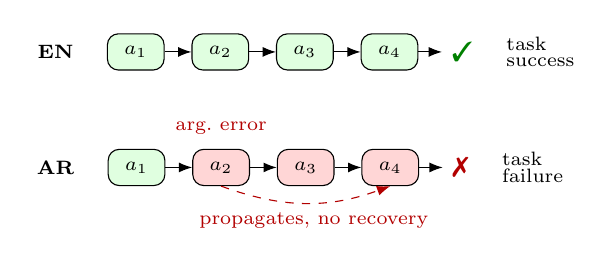
\begin{tikzpicture}[
  >=Latex,
  stepok/.style={draw, rounded corners, fill=green!12, minimum width=0.72cm, minimum height=0.46cm, font=\scriptsize, inner sep=1pt},
  stepbad/.style={draw, rounded corners, fill=red!16, minimum width=0.72cm, minimum height=0.46cm, font=\scriptsize, inner sep=1pt},
  lab/.style={font=\scriptsize\bfseries},
  node distance=0.34cm
]
% English track
\node[lab] (enl) {EN};
\node[stepok, right=0.30cm of enl] (e1) {$a_1$};
\node[stepok, right=of e1] (e2) {$a_2$};
\node[stepok, right=of e2] (e3) {$a_3$};
\node[stepok, right=of e3] (e4) {$a_4$};
\node[right=0.30cm of e4, green!50!black] (eok) {\ding{51}};
\draw[->] (e1)--(e2); \draw[->] (e2)--(e3); \draw[->] (e3)--(e4); \draw[->] (e4)--(eok);
% Non-English track
\node[lab, below=1.05cm of enl] (arl) {AR};
\node[stepok, right=0.30cm of arl] (a1) {$a_1$};
\node[stepbad, right=of a1] (a2) {$a_2$};
\node[stepbad, right=of a2] (a3) {$a_3$};
\node[stepbad, right=of a3] (a4) {$a_4$};
\node[right=0.30cm of a4, red!70!black] (afail) {\ding{55}};
\draw[->] (a1)--(a2); \draw[->] (a2)--(a3); \draw[->] (a3)--(a4); \draw[->] (a4)--(afail);
% annotations
\node[font=\scriptsize, text=red!70!black, align=center, above=0.06cm of a2] (err) {arg.\ error};
\draw[->, red!70!black, dashed] (a2.south) to[bend right=20] node[below, font=\scriptsize, pos=0.55] {propagates, no recovery} (a4.south);
\node[font=\scriptsize, align=left, right=0.18cm of eok] {task\\[-2pt]success};
\node[font=\scriptsize, align=left, right=0.18cm of afail] {task\\[-2pt]failure};
\end{tikzpicture}}
\captionof{figure}{One long-horizon multilingual failure pattern that motivates the
measurement. The same intent in English (top) and a non-English language
(bottom) differs in only one early step, an argument-level error at $a_2$, yet
that error can propagate and fail to recover. The paper asks where patterns of
this kind appear, where they do not, and whether they are better explained by
step-level weakness alone or by trajectory-level effects.}
\label{fig:teaser}

\end{center}

\section{Related Work}
\label{sec:related}

\paragraph{Multilingual tool calling.} \citet{mlcl2026} identify parameter-value
language mismatch in single-turn tool calls, while \citet{arabicenglish2026}
report related Arabic BFCL failures on complex and multi-step use. Their
``compounding language penalty'' is within-call stacking; we study
\emph{across-horizon} super-additivity against an independent-error null.
Multilingual multi-turn work reports context-retention brittleness
\citep{m2lingual2025}, and broader evaluation finds non-English gaps,
English-centric processing, and prompt-language effects
\citep{hada2024evaluators,fu2025reliable,singh2025globalmmlu,mexa2024,mahmood2026multilingualpromptlocalizationagentasajudge}.
Translate-test routes inputs through English \citep{shi2022language}; we use it
as a reference point while targeting a fixed, non-translated interface. None of
these studies measures super-additivity on execution-graded trajectories.

\paragraph{Long-horizon reliability and error propagation.} Multi-step tool use
degrades as horizons grow, motivating work on denoising, planning, reward
modeling, and confidence calibration
\citep{denoiseflow2026,phgpo2026,fintoolbench2026,planrewardbench2026,htc2026}.
\citet{turnwise2026} measure a multi-/single-turn gap, while
\citet{agentprop2026} measure propagation with controlled error injection;
other methods use explicit repair or self-distillation
\citep{structref2025,foundinconv2026}. This literature is monolingual; related
conversation work also observes early-turn derailment
\citep{laban2025lostinconversation}. We add the language axis and induce errors
naturally through user-language localization.

\paragraph{Executable tool-use benchmarks.} BFCL v3 uses state-based grading
\citep{patil2025bfcl}; $\tau$-bench and $\tau^2$-bench evaluate policy-adherent
multi-turn interaction \citep{yao2025taubench,barres2025tau2}; ToolBench and its
stable variant provide additional executable environments
\citep{qin2024toolbench,guo2024stabletoolbench}. We build on these evaluators
and add controlled localization.

\paragraph{Agentic evaluation generally.} Agent-as-a-Judge and related work
emphasize process-level, intermediate evaluation \citep{zhuge2025agentjudge}; we
rely instead on deterministic execution outcomes, which removes the judge from the
measurement loop entirely.

\section{Setup and Notation}
\label{sec:setup}

An agent solves a task $x$ by interacting with an environment over a trajectory of
steps. At step $k$ the agent emits a tool call $a_k$ (a function name and named
arguments), the environment executes it and returns an observation, and after
$K$ steps the environment reports a deterministic task outcome
$y \in \{0,1\}$ obtained by comparing the resulting system state to a gold state
\citep{patil2025bfcl,yao2025taubench}. We never use a model or a human to judge
the outcome.

Let $B$ be the set of backbones and $L$ the set of eight evaluation languages
(English, Arabic, Turkish, Chinese, Hindi, Japanese, Spanish, Swahili), spanning a
range of resource levels from higher-resource Spanish, Chinese, and Japanese to
lower-resource Turkish, Hindi, and Swahili. For a
task $x$ we hold the tool schemas fixed and English (language-invariant) and
localize only the user-facing query into language $\ell$, giving $x^{(\ell)}$.
This isolates the effect of the user's language at a fixed tool interface, the
realistic deployment condition.

The BFCL slice used in the main comparison contains four distinct multi-turn
tasks localized into eight languages, for $32$ task--language localized
queries in total. Each localized query is then executed under two decoding
seeds for Gemini 3 Flash Preview and Claude Sonnet 4.6, so every
backbone--language cell pools $8$ full-task trials ($4$ tasks $\times$ $2$
seeds) for $T(\ell,b)$ and $80$ isolated step replays ($10$ critical steps
$\times$ $4$ tasks $\times$ $2$ seeds) for $p(\ell,b)$. Task success is
therefore estimated over pooled task--seed trials rather than by averaging
seed-wise rates. Here a \emph{critical step} is an executable tool call in the
reference BFCL trajectory whose validity can be checked against the environment
and ordered gold call sequence; non-execution turns are not counted in $K$ or
in the replay-based $p(\ell,b)$.

For backbone $b$ and language $\ell$ we measure two things. The \textbf{task
success rate} is
\begin{equation}
T(\ell,b) = \Pr\nolimits_{x,s}[\, y = 1 \mid x^{(\ell)}, b, s\,],
\end{equation}
and the \textbf{single-turn validity rate} $p(\ell,b)$ is the probability that the
model emits a valid call for a critical step \emph{in isolation}: the step is
presented on its own with the correct (gold) preceding context, so no earlier
error can have propagated into it. This measures intrinsic per-step competence in
language $\ell$ \emph{without} any trajectory-level interaction. We obtain it by
replaying each critical step of a task as a single-turn query with gold history
(for BFCL v3 we additionally cross-check against its native single-turn
categories). We deliberately do \emph{not} use the marginal validity
of calls emitted during the full trajectory, because that marginal already absorbs
propagated errors and would make the compounding test below circular. If
$N_{\ell,b}$ denotes the number of pooled task--seed trials, and
$M_{\ell,b}$ the number of isolated replayed steps, the reported empirical
rates are the add-one-smoothed estimates
\[
\hat T(\ell,b)=\frac{1+\sum_{i=1}^{N_{\ell,b}}y_i}{2+N_{\ell,b}},
\qquad
\hat p(\ell,b)=\frac{1+\sum_{j=1}^{M_{\ell,b}}v_j}{2+M_{\ell,b}}.
\]
Here $p(\ell,b)$ is the corresponding probability over pooled
task--step--seed replay trials. We use $\hat T$ and $\hat p$ as $T$ and $p$ in
the displayed metric equations. The uncertainty analysis uses $200$ bootstrap
resamples of task--seed clusters; because the run label is part of the cluster
identifier, the resampling unit is task--seed rather than task alone. The small
number of underlying tasks makes the resulting intervals and adjusted p-values
coarse.

\section{Does the Per-Step Penalty Compound?}
\label{sec:compound}

\subsection{An independent-error null}
The question is whether the task-level cross-lingual gap is larger than the
per-step gap predicts. We make ``predicts'' precise with a null in which step
errors are independent.

\begin{proposition}[Independent-error prediction]
\label{prop:indep}
Suppose a task of effective length $K$ succeeds only if every critical step is
valid, and suppose step validity events are mutually independent with common
per-step validity $p(\ell,b)$. Then the task success rate is
$T_{\mathrm{ind}}(\ell,b) = p(\ell,b)^{K}$, and the cross-lingual task-success
ratio relative to English is
\begin{equation}
\frac{T_{\mathrm{ind}}(\ell,b)}{T_{\mathrm{ind}}(\mathrm{EN},b)}
= \left(\frac{p(\ell,b)}{p(\mathrm{EN},b)}\right)^{K}.
\label{eq:indep}
\end{equation}
\end{proposition}

\noindent The proof is immediate (Appendix~\ref{app:indep}) and the proposition is
deliberately modest; its role is to provide a falsifiable baseline. Equation \eqref{eq:indep} says that under independence a per-step validity ratio
close to one is amplified only geometrically by the horizon $K$. Writing the
observed and predicted task-success ratios relative to English as
$r_{\mathrm{obs}}(\ell,b)=T(\ell,b)/T(\mathrm{EN},b)$ and
$r_{\mathrm{ind}}(\ell,b)=T_{\mathrm{ind}}(\ell,b)/T_{\mathrm{ind}}(\mathrm{EN},b)$,
we define the \textbf{compounding factor}
\begin{equation}
\mathrm{CF}(\ell,b) =
\frac{\log r_{\mathrm{obs}}(\ell,b)}{\log r_{\mathrm{ind}}(\ell,b)},
\label{eq:cf}
\end{equation}
the ratio of observed to independence-predicted log task-success degradation.
$\mathrm{CF}\approx 1$ means the trajectory composes as if steps were independent
at their single-turn competence; $\mathrm{CF}>1$ means \emph{super-additive
compounding}: observed multi-turn success is lower than the independent
composition of single-turn competence predicts, so the non-English task-level
deficit is worse than its single-turn per-step gap can explain, the signature of
cross-step interactions such as error propagation.
$K$ is estimated per environment from reference trajectory lengths; our analysis
evaluates $K\in\{9,10,11\}$ around the rounded mean.

Here $K$ should be read as an \emph{effective horizon proxy}, not as a literal
count of independent Bernoulli trials. BFCL trajectories contain shared
prefixes, dependencies, and opportunities for repair, so the common null is too
crude as an absolute model of task success. That absolute misfit is visible even
in English: at $K=10$, the common null predicts $T_{\mathrm{ind}}(\mathrm{EN}) =
0.237$ for Gemini 3 Flash Preview and $0.272$ for Claude Sonnet 4.6, versus
observed $T(\mathrm{EN}) = 0.900$ and $0.700$. We therefore use the null
primarily through the cross-lingual ratio $r_{\mathrm{ind}}$, where the
English-side task difficulty partly cancels within a backbone, and we
cross-check robustness with the position-specific null in
Appendix~\ref{app:indep}. Under the common null, $\mathrm{CF}=K^\star/K$ where
$K^\star(\ell,b)=\log r_{\mathrm{obs}}(\ell,b)\,/\,
\log\!\bigl(p(\ell,b)/p(\mathrm{EN},b)\bigr)$ is the crossover horizon at which
the observed and null-predicted cross-lingual degradations match. For Turkish
on Gemini 3 Flash Preview, $K^\star=12.44$, placing the reference $K=10$
on the beyond-null side of the crossover.

The ratio in Eq.~\eqref{eq:cf} is unstable when $\log r_{\mathrm{ind}}$ is near
zero (a negligible per-step gap) or when a task-success rate is near $0$ or $1$.
We therefore (i) apply add-one smoothing to all rates before taking logs, (ii)
restrict the ratio to cells where $r_{\mathrm{ind}}$ is bounded away from $1$ and
report the rest separately, and (iii) report the robust additive complement, the
\emph{excess log-degradation}
$\Delta(\ell,b)=\log r_{\mathrm{obs}}(\ell,b)-\log r_{\mathrm{ind}}(\ell,b)$,
which is well defined throughout and for which $\Delta<0$ is the same
super-additivity test as $\mathrm{CF}>1$. We report both and base conclusions on
their agreement. Crucially, $\mathrm{CF}>1$ (equivalently $\Delta<0$) is
\emph{necessary but not sufficient} evidence of true propagation, because it can
also arise from per-step difficulty that is heterogeneous and correlated within a
task; the propagation and recovery analysis below, computed at matched per-step
validity, is what we use to separate genuine propagation from heterogeneity.

\begin{center}
\resizebox{0.97\columnwidth}{!}{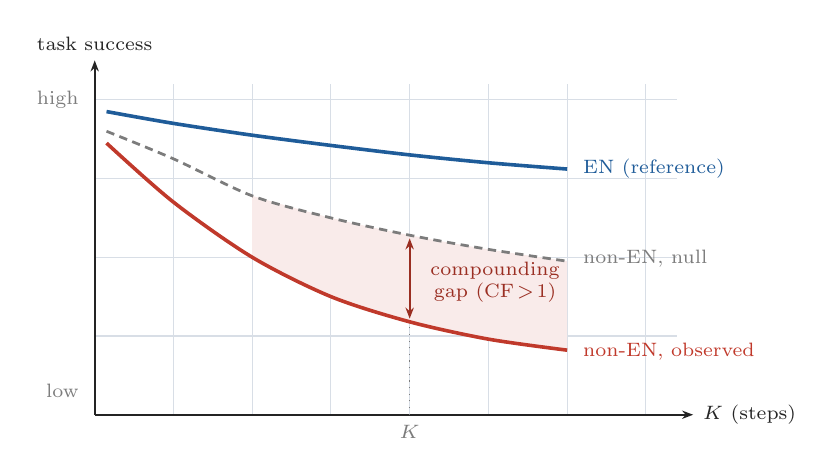
\begin{tikzpicture}[x=1cm, y=1cm]
  % gridlines
  \foreach \y in {1,2,3,4}{\draw[gridln] (0,\y)--(7.4,\y);}
  \foreach \x in {1,2,3,4,5,6,7}{\draw[gridln] (\x,0)--(\x,4.2);}
  % axes
  \draw[axis] (0,0)--(7.6,0) node[right, font=\scriptsize, text=cInk] {$K$ (steps)};
  \draw[axis] (0,0)--(0,4.5) node[above, font=\scriptsize, text=cInk] {task success};
  \node[tick, anchor=east] at (-0.08,4.0) {high};
  \node[tick, anchor=east] at (-0.08,0.3) {low};
  % shaded compounding gap
  \fill[cBad!10]
    plot[smooth] coordinates {(2,2.78)(3,2.5)(4,2.28)(5,2.1)(6,1.95)} --
    plot[smooth] coordinates {(6,0.82)(5,0.96)(4,1.18)(3,1.5)(2,2.0)} -- cycle;
  % EN (reference) curve
  \draw[cRef, line width=1.3pt]
    plot[smooth] coordinates {(0.15,3.85)(1,3.7)(2,3.55)(3,3.42)(4,3.3)(5,3.2)(6,3.12)};
  % non-EN predicted under independence
  \draw[cMut, line width=1.0pt, dash pattern=on 3pt off 2pt]
    plot[smooth] coordinates {(0.15,3.6)(1,3.25)(2,2.78)(3,2.5)(4,2.28)(5,2.1)(6,1.95)};
  % non-EN observed (super-additive)
  \draw[cBad, line width=1.3pt]
    plot[smooth] coordinates {(0.15,3.45)(1,2.7)(2,2.0)(3,1.5)(4,1.18)(5,0.96)(6,0.82)};
  % direct curve labels
  \node[font=\scriptsize, anchor=west, text=cRef] at (6.08,3.12) {EN (reference)};
  \node[font=\scriptsize, anchor=west, text=cMut] at (6.08,1.98) {non-EN, null};
  \node[font=\scriptsize, anchor=west, text=cBad] at (6.08,0.80) {non-EN, observed};
  % compounding gap callout
  \draw[{Stealth[length=4pt]}-{Stealth[length=4pt]}, line width=0.7pt, cBad!80!black] (4,2.24)--(4,1.22);
  \node[font=\scriptsize, align=center, anchor=south west, text=cBad!80!black] at (4.14,1.30)
    {compounding\\gap ($\mathrm{CF}\!>\!1$)};
  \draw[dotted, cMut] (4,0)--(4,1.18);
  \node[tick] at (4,-0.22) {$K$};
\end{tikzpicture}}
\captionof{figure}{Illustrative schematic (not measured data). As the trajectory
length $K$ grows, the independence null predicts only a mild non-English drop
(gray dashed). The hypothesis this paper tests is that the observed non-English
curve (red) falls faster, so the gap to the null widens with $K$ (super-additive
compounding, $\mathrm{CF}>1$). Section~\ref{sec:experiments} quantifies this gap;
Figure~\ref{fig:results} reports it on the measured data.}
\label{fig:compound}

\end{center}

\subsection{Where the gap originates}
We label every invalid step of every trajectory with one of three step-level
stages and an associated failure type: (i) \emph{intent and tool selection}
(wrong function chosen), (ii) \emph{argument and parameter formatting} (right
function, invalid or language-mismatched arguments, the single-turn mode of
\citet{mlcl2026}), and (iii) \emph{sequencing and planning} (valid calls in the
wrong order or missing a prerequisite). Stage labels are derived
programmatically from the execution trace and the reference, not by a judge:
missing or unparseable calls, and wrong functions not appearing elsewhere in
the task's gold sequence, map to intent/selection; same-function argument
mismatches map to argument/parameter unless BFCL reports a state/context
mismatch; and calls whose function appears elsewhere in the task's gold
sequence map to sequencing/planning.
Recovery is then reported separately as a trajectory-level effect rather than as
another per-step taxonomy bucket.

Two quantities isolate trajectory-level behavior that is invisible in single-turn
replays. The \textbf{detour-to-failure rate} is the probability that a trajectory
ends unsuccessfully conditional on an off-reference detour; the complementary
\textbf{post-detour recovery rate} is the probability that it eventually
succeeds. We operationalize these quantities by greedily aligning the emitted
call sequence to the ordered gold call sequence: an emitted call that does not
match the next unmatched gold call marks an off-reference detour, and later
success or failure determines the corresponding trajectory outcome. These
quantities should therefore be read as detour-conditioned propagation and
recovery indicators, not as a causal estimate tied to the first invalid step.
The hypothesis is that non-English trajectories have higher detour-to-failure
and lower post-detour recovery rates even at matched per-step validity, a
pattern consistent with trajectory-level amplification.

\section{Conditional Mitigation Design: Language-Invariant Argument Canonicalization}
\label{sec:method}

If argument or parameter mismatches propagate, a schema-boundary layer could
canonicalize values before execution and return a structured English recovery
hint after an environment error \citep{mlcl2026}. The proposed layer is
model-agnostic, requires no fine-tuning, and would be judged only by execution
success; its pseudocode appears in Appendix~\ref{app:method}.
\paragraph{Follow-up comparison.} Translate-test routes the full query through
English, while self-repair retries after an error with a generic reflection
prompt. Both are reference controls rather than deployment-faithful competitors:
the first changes the user-to-interface contract and the second adds retries.
These are proposed follow-up experiments, not reported results; canonicalization
would be justified only by a net task-success gain.

\section{Experiments}
\label{sec:experiments}

The evidence base is BFCL-only. Estimation uses task--seed cluster bootstrap
and multiple decoding seeds; significance uses Holm--Bonferroni correction.
Full per-experiment protocols (metrics, estimands, and analysis scope) are in
Appendix~\ref{app:protocol}.

\begin{itemize}
\itemsep0.15em
\item BFCL evidence base: localize BFCL v3 multi-turn queries into
the eight languages, validate with back-translation and reference-call
invariance, run the two backbone configurations with usable English baselines,
and record full execution traces,
per-step validity $p(\ell,b)$, and task success $T(\ell,b)$.
\item BFCL compounding analysis: compute the compounding factor
$\mathrm{CF}(\ell,b)$ (Eq.~\ref{eq:cf}) and excess log-degradation
$\Delta(\ell,b)$ with uncertainty over $K\in\{9,10,11\}$.
\item BFCL decomposition: classify failure stages and estimate
detour-to-failure and post-detour recovery rates by language at matched
per-step validity.
\item Proposed follow-up: apply canonicalization and
canonicalization-plus-recovery, and the translate-test and self-repair
baselines, only if the decomposition identifies a mechanism that plausibly
matches a tool-boundary fix.
\item BFCL robustness: translation-confound controls and BFCL-scope robustness
(seeds, $K$ sensitivity, leave-one-language-out, and fidelity filtering), with
broader environment coverage treated as future work and outside the scope of
this study.
\end{itemize}

\paragraph{Reproducibility.} The repository contains the localized query sets and
fidelity ratings, full execution traces, the stage-labeling and metric code
(including $\mathrm{CF}$ and $\Delta$), and a pinned BFCL checkout. The
canonicalization layer is described as a follow-up design rather than reported
as an evaluated result.

\section{Results}
\label{sec:results}

We first ask whether any backbone--language cell shows directional evidence
beyond the independent-error null, then whether detour-conditioned outcomes
reveal behavior not reducible to step-frequency differences. The mitigation
design is discussed only as a mechanism-aligned follow-up because it was not
evaluated in this study.

Figure~\ref{fig:results} visualizes the per-cell compounding factors summarized
in Table~\ref{tab:cf}; the Chinese/Gemini marker lies at the null within
rounding, whereas Turkish/Gemini is the only clearly directional marker above
it.

Table~\ref{tab:cf} shows that the BFCL results do not support a universal
compounding claim. Gemini 3 Flash Preview provides the strongest directional
signal:
its English baseline is strong ($p=0.866$, $T=0.900$), and Turkish is the
strongest beyond-null cell ($p=0.793$, $T=0.300$, $\mathrm{CF}=1.244$ at
$K=10$), but it does not meet the Holm threshold under the $200$-resample
procedure used here.
Chinese is effectively at the null
($\mathrm{CF}=1.000$), while Arabic, Spanish, Hindi, Japanese, and Swahili all
remain below that level. Claude Sonnet 4.6 is stable and multilingual, but its
non-English cells stay modest throughout ($\mathrm{CF}=0.066$ to $0.547$). We
therefore restrict the primary comparison to these two backbones, which provide
usable English reference baselines. The common null is informative here only as a
relative baseline, not as an absolute English success model: at $K=10$ it
predicts $T_{\mathrm{ind}}(\mathrm{EN})=0.237$ for Gemini 3 Flash Preview and
$0.272$ for Claude Sonnet 4.6, versus observed $T(\mathrm{EN})=0.900$ and
$0.700$. This is why the main quantity of interest is the cross-lingual ratio
after English cancellation, with the position-specific null reported as a
robustness check rather than a replacement claim.

\begin{center}

\centering\small
\setlength{\tabcolsep}{5pt}
\resizebox{\columnwidth}{!}{\begin{tabular}{llrrrr}
\toprule
 & & \multicolumn{2}{c}{Per-cell rates} & \multicolumn{2}{c}{Cross-lingual, vs.\ null} \\
\cmidrule(lr){3-4}\cmidrule(lr){5-6}
Backbone & Lang. & $p(\ell,b)$ & $T(\ell,b)$ & $\mathrm{CF}(\ell,b)$ & $\Delta(\ell,b)$ \\
\midrule
\multirow{8}{*}{Gemini 3 Flash Preview}
 & EN & 0.866 & 0.900 & \cellcolor{black!8}ref. & \cellcolor{black!8}ref. \\
 & AR & 0.646 & 0.100 & \cellcolor{cRef!9}0.751  & $+0.73$ \\
 & ES & 0.768 & 0.500 & \cellcolor{cRef!17}0.492 & $+0.61$ \\
 & HI & 0.768 & 0.500 & \cellcolor{cRef!17}0.492 & $+0.61$ \\
 & JA & 0.720 & 0.500 & \cellcolor{cRef!23}0.317 & $+1.26$ \\
 & SW & 0.622 & 0.100 & \cellcolor{cRef!12}0.664 & $+1.11$ \\
 & TR & 0.793 & 0.300 & \cellcolor{cBad!14}\textbf{1.244} & $\mathbf{-0.22}$ \\
 & ZH & 0.695 & 0.100 & \cellcolor{cRef!1}1.000  & $+0.00$ \\
\cmidrule(l){2-6}
\multirow{8}{*}{Claude Sonnet 4.6}
 & EN & 0.878 & 0.700 & \cellcolor{black!8}ref. & \cellcolor{black!8}ref. \\
 & AR & 0.671 & 0.500 & \cellcolor{cRef!30}0.125 & $+2.35$ \\
 & ES & 0.854 & 0.600 & \cellcolor{cRef!15}0.547 & $+0.12$ \\
 & HI & 0.695 & 0.600 & \cellcolor{cRef!32}0.066 & $+2.18$ \\
 & JA & 0.805 & 0.600 & \cellcolor{cRef!28}0.177 & $+0.71$ \\
 & SW & 0.622 & 0.200 & \cellcolor{cRef!22}0.363 & $+2.19$ \\
 & TR & 0.780 & 0.600 & \cellcolor{cRef!30}0.131 & $+1.03$ \\
 & ZH & 0.707 & 0.400 & \cellcolor{cRef!25}0.259 & $+1.61$ \\
\bottomrule
\end{tabular}}
\captionof{table}{Per-step validity $p$, task success $T$, compounding factor
$\mathrm{CF}$, and excess log-degradation $\Delta$ at the rounded BFCL horizon
$K=10$ for the two interpretable backbones. Grouped per-cell rates on the left, cross-lingual deviation from the
null on the right, with CF cells shaded by distance from $\mathrm{CF}=1$ (blue
for $\mathrm{CF}<1$, red for $\mathrm{CF}>1$). Each backbone--language cell
pools $8$ full-task trials ($4$ tasks $\times$ $2$ seeds) and $80$ isolated
step replays; displayed values are computed from the pooled smoothed counts.
Under the $200$-resample procedure used here, no non-English cell meets the Holm
threshold for $\mathrm{CF}>1$.
Appendix Table~\ref{tab:cf_ci_appendix} reports the corresponding 95\%
bootstrap CIs and Holm-adjusted p-values for each non-English cell. Under the
$200$-resample procedure, these adjusted values are coarse summaries for
the four-task slice, not evidence of equivalence.}
\label{tab:cf}

\end{center}

\begin{center}
\resizebox{\columnwidth}{!}{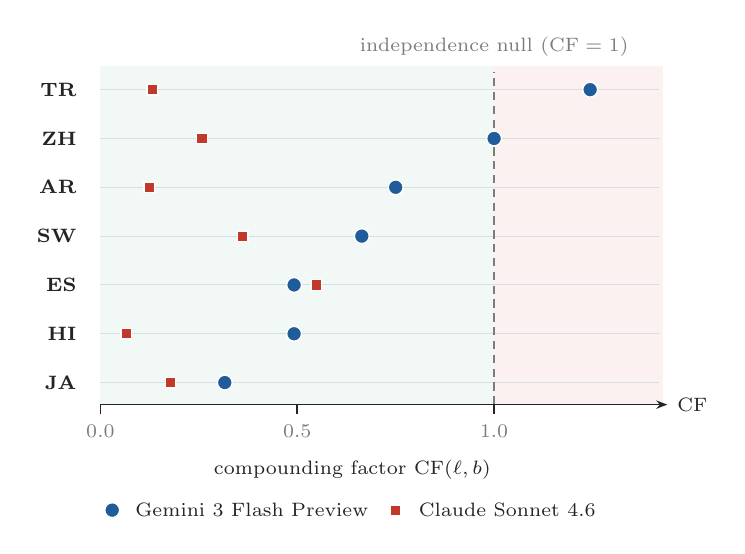
\begin{tikzpicture}[x=1cm,y=1cm,
  gmk/.style={circle, fill=cRef, draw=white, line width=0.5pt, inner sep=1.9pt},
  cmk/.style={rectangle, fill=cBad, draw=white, line width=0.5pt, minimum size=3.8pt, inner sep=0pt},
  glab/.style={font=\scriptsize\bfseries, text=cInk, anchor=east},
  plab/.style={font=\scriptsize, text=cInk}]
  \fill[cGood!6] (0,-0.28) rectangle (5.0,4.02);
  \fill[cBad!7]  (5.0,-0.28) rectangle (7.15,4.02);
  \foreach \y in {0,0.62,1.24,1.86,2.48,3.10,3.72}{\draw[gridln](0,\y)--(7.1,\y);}
  \draw[cMut,line width=1.0pt,dash pattern=on 3pt off 2pt](5.0,-0.28)--(5.0,3.95);
  \node[font=\scriptsize,text=cMut,anchor=south] at (5.0,4.02) {independence null ($\mathrm{CF}=1$)};
  \draw[axis](0,-0.28)--(7.2,-0.28) node[right,font=\scriptsize,text=cInk]{$\mathrm{CF}$};
  \foreach \tx/\tl in {0/0.0,2.5/0.5,5.0/1.0}{\draw[axis,-](\tx,-0.28)--(\tx,-0.40);\node[tick,anchor=north]at(\tx,-0.42){\tl};}
  \node[font=\scriptsize,text=cInk,anchor=north] at (3.2,-0.86) {compounding factor $\mathrm{CF}(\ell,b)$};
  \node[glab] at (-0.18,3.72) {TR}; \node[gmk] at (6.22,3.72){}; \node[cmk] at (0.66,3.72){};
  \node[glab] at (-0.18,3.10) {ZH}; \node[gmk] at (5.00,3.10){}; \node[cmk] at (1.29,3.10){};
  \node[glab] at (-0.18,2.48) {AR}; \node[gmk] at (3.75,2.48){}; \node[cmk] at (0.62,2.48){};
  \node[glab] at (-0.18,1.86) {SW}; \node[gmk] at (3.32,1.86){}; \node[cmk] at (1.81,1.86){};
  \node[glab] at (-0.18,1.24) {ES}; \node[gmk] at (2.46,1.24){}; \node[cmk] at (2.74,1.24){};
  \node[glab] at (-0.18,0.62) {HI}; \node[gmk] at (2.46,0.62){}; \node[cmk] at (0.33,0.62){};
  \node[glab] at (-0.18,0.00) {JA}; \node[gmk] at (1.58,0.00){}; \node[cmk] at (0.89,0.00){};
  \node[gmk] at (0.15,-1.62){}; \node[plab,anchor=west] at (0.32,-1.62){Gemini 3 Flash Preview};
  \node[cmk] at (3.75,-1.62){}; \node[plab,anchor=west] at (3.92,-1.62){Claude Sonnet 4.6};
\end{tikzpicture}}
\captionof{figure}{Compounding factor by language for the two interpretable
backbones (measured data, Table~\ref{tab:cf}; one marker per cell, $K=10$).
The dashed line is the independence null. Turkish on Gemini 3 Flash Preview is
the only cell materially above the null; Chinese is visually at the null within
rounding. Appendix Table~\ref{tab:cf_ci_appendix} reports the pointwise
uncertainty and Holm-adjusted significance values.}
\label{fig:results}
\end{center}


\begin{center}

\centering\small
\setlength{\tabcolsep}{6pt}
\begin{tabular}{lrrr}
\toprule
Stage / effect & EN & non-EN & $\delta_{\mathrm{stage}}$ \\
\midrule
\multicolumn{4}{l}{\textit{Failure-type mix (share of invalid steps)}}\\
\addlinespace[1pt]
Intent / selection    & 0.579 & 0.440 & $-0.14$ \\
Argument / parameter  & 0.000 & 0.298 & $+0.30$ \\
Sequencing / planning & 0.421 & 0.262 & $-0.16$ \\
\midrule
\multicolumn{4}{l}{\textit{Trajectory-level effects (matched $8/10$, $9/10$ bins)}}\\
\addlinespace[1pt]
Detour-to-failure rate & 0.143 & 0.353 & \cellcolor{cBad!16}$+0.21$ \\
Post-detour recovery   & 0.857 & 0.647 & \cellcolor{cBad!16}$-0.21$ \\
\bottomrule
\end{tabular}
\captionof{table}{Where the gap originates (failure-type mix, top block) and the
two trajectory-level effects (bottom block), English vs.\ non-English pooled
over the two main backbones; $\delta_{\mathrm{stage}}$ is non-EN minus EN.
The detour-conditioned rates are computed on the shared replay-validity bins so
the comparison is not merely about error frequency; the shaded rows indicate
the directional non-English disadvantage (more detour-to-failure, less
post-detour recovery). The displayed rates are weighted matched-bin estimates.
The corresponding pooled raw detour-to-failure counts are $2/15$ English
(Wilson 95\% CI $[0.037, 0.379]$) versus $22/49$ non-English
($[0.319, 0.587]$), with unadjusted Fisher two-sided $p=0.034$; the
complementary recovery counts are $13/15$ English ($[0.621, 0.963]$) versus
$27/49$ non-English ($[0.413, 0.681]$). We therefore treat this pattern as
descriptive rather than as a standalone established effect.}
\label{tab:stage}

\end{center}

The effective-horizon choice also matters. Across the supported sweep
$K\in\{9,10,11\}$, Turkish on Gemini remains the strongest directional cell
($\mathrm{CF}=1.38$, $1.24$, and $1.13$, respectively), while Chinese moves
from just above the null at $K=9$ to below it at $K=11$. Under the common null,
Turkish/Gemini has $K^\star=12.44$, so the reference $K=10$ lies on the
beyond-null side of the crossover. We therefore treat the signal as
$K$-sensitive rather than robust and retain $K=10$ as the reference length
proxy for the main table. Appendix Table~\ref{tab:headline_task_breakdown}
shows that the headline Turkish/Gemini directional signal is also not uniform
across the four BFCL tasks, which is another reason we avoid a stronger
aggregate claim.

GPT-4o (\emph{gpt-4o-2024-08-06}) is excluded from Table~\ref{tab:cf} because
it never supplied a usable English reference backbone on BFCL: on the OpenRouter
run it achieved $0/8$ English task successes with $58/80$
replay-valid steps, and a direct OpenAI diagnostic also gave $0/4$ English
task successes with $27/40$ replay-valid steps.
Backbone inclusion is therefore an English-baseline usability restriction, not a
claim that the omitted model is representative of frontier systems. The main
conclusions generalize only to the two interpretable backbones and this BFCL
slice.

Table~\ref{tab:stage} is best read descriptively. The non-English failure mix is not purely
argument-boundary driven: intent/selection errors are the largest share
($0.440$), with argument/parameter ($0.298$) and sequencing/planning ($0.262$)
close behind. After matching on replay-validity bins, non-English trajectories
end in failure after off-reference detours more often ($0.353$ vs.\ $0.143$)
and recover less often ($0.647$ vs.\ $0.857$). Because the weighted estimator
and pooled raw-count test answer different questions, both are descriptive
evidence that the gap is not only a per-step frequency story.

We do not evaluate the canonicalization intervention because the
headline cells do not expose an argument-boundary-dominated failure mechanism
that the proposed layer is designed to fix. For
Turkish on Gemini 3 Flash Preview, the replay failure mix is $62.5\%$
intent/selection and $37.5\%$ sequencing/planning, with no
argument/parameter dominance. For Turkish on Claude Sonnet 4.6, the split is
$82.4\%$ intent/selection and $17.6\%$ argument/parameter. Some secondary cells
are more argument-heavy (Arabic and Swahili on Gemini 3 Flash Preview, and
Chinese on Claude Sonnet 4.6), but those are not the main carriers of the
headline interpretation. The five-setting mitigation matrix is therefore left
as a targeted follow-up rather than a reported contribution.

The BFCL-scope robustness checks leave the heterogeneity conclusion intact. All $32/32$
localized queries pass reference-call invariance; at the fidelity threshold
(rating $\ge 3$), the low-fidelity filter removes no BFCL examples;
the $K \in \{9,10,11\}$ sensitivity sweep preserves the main interpretation
once the position-specific null is included; and leave-one-language-out never
produces a cell meeting the Holm threshold under the $200$-resample procedure.
When Turkish is present, Turkish on Gemini 3 Flash Preview remains the strongest
directional beyond-null cell; when Turkish is held out, Chinese on Gemini 3
Flash Preview becomes the strongest directional cell, still without significance
at the reference $K=10$. Seed variance changes magnitudes
but not the main interpretation.

\section{Discussion}
\label{sec:discussion}
Our results reframe multilingual agent reliability as a heterogeneity problem
over the horizon rather than a universal compounding law. What matters for
deployment is not only how often a single non-English call is valid, but which
backbones and languages turn step-level weakness into trajectory-level failure
and which do not. On the BFCL slice, the strongest directional
beyond-null evidence comes from Turkish on Gemini 3 Flash Preview, but no cell
meets the Holm threshold under the $200$-resample procedure. The more
stable statement is therefore not ``all multilingual
tool use compounds,'' but ``some multilingual long-horizon regimes show
trajectory effects that step accuracy alone does not explain.''

The detour-conditioned analysis identifies the practical lever: prevention is
plausible when argument or sequencing failures propagate, but a thin interface
fix may do little when weaker step competence dominates. In this slice,
intent/selection and sequencing are at least as important as parameter
formatting, and the headline Turkish/Gemini cell has no dominant
argument/parameter mode. A call--execute intervention is therefore conditional
on the failure mix; translate-test remains an upper reference because it changes
the user-to-interface contract.

The claim is correspondingly scoped: some regimes show trajectory degradation
beyond a step-level null, others do not, and backbone stability matters. GPT-4o
(\emph{gpt-4o-2024-08-06}) never yielded a usable English BFCL baseline under
either serving path tested, so it is excluded from the main comparison rather
than averaged away.

\section{Conclusion}
\label{sec:conclusion}
We study multilingual reliability where it matters for agents, over a long
horizon, with execution ground truth and human review limited to query
localization. The BFCL evidence does not support a single universal compounding
story. Instead, it
shows heterogeneous multilingual long-horizon behavior across backbones and
languages, which must be explained with trajectory-level decomposition rather
than with step accuracy alone. In this BFCL evidence base, no
non-English cell meets the Holm threshold for $\mathrm{CF}>1$ under the
$200$-resample procedure, but the
matched-validity detour-conditioned analysis still points in the same
direction, with non-English trajectories recovering less reliably after going
off reference. The paper's main result is therefore a constrained one: on this
BFCL slice, multilingual long-horizon degradation is heterogeneous, $K$-sensitive,
and not exhausted by step accuracy alone.

\section*{Limitations}
Coverage is limited to BFCL v3 multi-turn, eight languages, and four tasks with
two seeds: each cell has $8$ full-task trials and $80$ isolated replays, making
estimates sensitive to individual outcomes. The effective horizon is a proxy,
so we report $K\in\{9,10,11\}$. Queries are machine-assisted and
human-reviewed; all $32/32$ localizations pass reference-call invariance and
none are filtered, so this robustness check cannot stress the claim with a
substantial excluded subset. The proposed mitigation is untested. English,
language-invariant schemas match a common deployment setting but not localized
interfaces, and broader environment coverage remains future work.

\section*{Ethics Statement}
This work uses no human subjects and no personal data. All model runs use
commercial or open APIs under their terms. Multilingual reliability has direct
fairness implications: agents that are markedly less reliable in non-English
languages disadvantage those users, which is the problem this paper measures and
seeks to reduce. Query localization for low-resource languages should be reviewed
by competent speakers; we report which languages received native review. The
authors verify and take responsibility for all content, including
Proposition~\ref{prop:indep} and the proposed mitigation; AI assistance in
drafting is disclosed in accordance with venue policy.

\bibliography{references}

\appendix

\section{Proof of Proposition~\ref{prop:indep}}
\label{app:indep}
If a task succeeds only when each of $K$ critical steps is valid and step validity
events $V_1,\dots,V_K$ are independent with $\Pr[V_k=1]=p(\ell,b)$, then
$T_{\mathrm{ind}}(\ell,b)=\Pr[\bigcap_k V_k]=\prod_k \Pr[V_k]=p(\ell,b)^K$, and the
cross-lingual ratio in Eq.~\eqref{eq:indep} follows by dividing the two
expressions. Taking logs of the observed and predicted ratios and dividing gives the
compounding factor in Eq.~\eqref{eq:cf}; $\mathrm{CF}=1$ exactly under the null,
and $\mathrm{CF}>1$ means observed multi-turn success falls below the independent
product of single-turn competence, i.e., cross-step interactions (propagation of
early errors, degraded state tracking) reduce success below the no-interaction
baseline. This is necessary but not sufficient for error propagation
specifically, since other cross-step interactions could also lower success: we
therefore recompute the prediction with step-position-specific single-turn
validity $\prod_k p_k$, which removes heterogeneity across positions, and rely on
the matched-validity propagation and recovery analysis (Section~\ref{sec:compound},
the decomposition analysis) to isolate propagation. As discussed in the main
text, the common null is not treated as an absolute model of English success:
at $K=10$ it underpredicts English BFCL task success for both Gemini 3 Flash
Preview ($0.237$ vs.\ $0.900$) and Claude Sonnet 4.6 ($0.272$ vs.\ $0.700$).
Its role is relative, after English cancellation within a backbone. We report
whether the $\mathrm{CF}>1$ test is unchanged under the position-specific null
rather than assuming it.

\section{Supplementary Quantitative Tables}
\label{app:supp}

\begin{center}
\centering\small
\setlength{\tabcolsep}{6pt}
\resizebox{\columnwidth}{!}{\begin{tabular}{llccc}
\toprule
Backbone & Lang. & $\mathrm{CF}$ & 95\% CI & $p_{\mathrm{Holm}}$ \\
\midrule
\multirow{7}{*}{Gemini 3 Flash Preview}
 & AR & 0.751 & [0.641, 0.888] & 1.000 \\
 & ES & 0.492 & [0.101, 1.221] & 1.000 \\
 & HI & 0.492 & [0.097, 0.955] & 1.000 \\
 & JA & 0.317 & [0.100, 0.663] & 1.000 \\
 & SW & 0.664 & [0.542, 0.816] & 1.000 \\
 & TR & 1.244 & [0.573, 3.679] & 1.000 \\
 & ZH & 1.000 & [0.847, 1.226] & 1.000 \\
\cmidrule(l){2-5}
\multirow{7}{*}{Claude Sonnet 4.6}
 & AR & 0.125 & [0.000, 0.349] & 1.000 \\
 & ES & 0.547 & [0.000, 4.262] & 1.000 \\
 & HI & 0.066 & [0.000, 0.227] & 1.000 \\
 & JA & 0.177 & [0.000, 0.927] & 1.000 \\
 & SW & 0.363 & [0.172, 0.650] & 1.000 \\
 & TR & 0.131 & [0.000, 0.987] & 1.000 \\
 & ZH & 0.259 & [0.059, 0.762] & 1.000 \\
\bottomrule
\end{tabular}}
\captionof{table}{Supplement to Table~\ref{tab:cf}: per-cell 95\% bootstrap
confidence intervals for $\mathrm{CF}$ and Holm-adjusted one-sided p-values for
$\Delta<0$ (equivalently $\mathrm{CF}>1$) at the reference $K=10$. The main
results table hides these quantities; this appendix table makes the underlying
uncertainty explicit. Because the resampling units are task--seed clusters and
the number of underlying tasks is small, these intervals and adjusted values
are descriptive uncertainty summaries rather than decisive evidence.}
\label{tab:cf_ci_appendix}
\end{center}

\begin{center}
\centering\small
\setlength{\tabcolsep}{5pt}
\resizebox{\columnwidth}{!}{\begin{tabular}{lrrrrrr}
\toprule
Task & EN $p$ & EN $T$ & TR $p$ & TR $T$ & TR $\Delta$ & TR $\mathrm{CF}$ \\
\midrule
Base & 0.864 & 0.750 & 0.773 & 0.750 & +1.112 & -- \\
Miss-func & 0.773 & 0.750 & 0.773 & 0.250 & $-1.099$ & -- \\
Miss-param & 0.864 & 0.750 & 0.773 & 0.250 & +0.014 & 0.988 \\
Long-context & 0.864 & 0.750 & 0.773 & 0.250 & +0.014 & 0.988 \\
\bottomrule
\end{tabular}}
\captionof{table}{Per-task descriptive breakdown for the headline Turkish on
Gemini 3 Flash Preview comparison against its task-matched English reference at
$K=10$. Each row pools two seeds for one BFCL task, so $T$ is estimated from
two full-task trials and $p$ from $20$ isolated step replays. This reveals that
the aggregate Turkish/Gemini signal is not uniform across tasks. $\mathrm{CF}$
is omitted when the observed task-level log gap is zero or the task-specific
independent baseline ratio is numerically at the null
($\log r_{\mathrm{ind}} \approx 0$), the same instability regimes discussed in
Section~\ref{sec:compound}.}
\label{tab:headline_task_breakdown}
\end{center}

\section{Per-Experiment Protocol}
\label{app:protocol}
Task and step outcomes are execution-scored; human review is used only for
query localization and fidelity checks.

\paragraph{Localization.} Source: BFCL v3 multi-turn tasks used in this study.
Procedure: localize each user-facing query into the
eight languages with machine translation plus competent-speaker review; keep all
tool schemas and reference solutions in English. Validate with independent
back-translation and a reference-call invariance check (the gold call sequence
must be unchanged by localization). Output: localized query sets and a per-query
fidelity rating. Reduces: the translation-confound objection.

\paragraph{BFCL runs.} Execute the selected backbone set on every localized task
with the official executable evaluator and available decoding seeds. Record full
multi-turn traces and task success $T(\ell,b)$. \emph{Separately} measure the
single-turn validity $p(\ell,b)$ by replaying each critical step in isolation with
gold preceding context (Section~\ref{sec:setup}); do not read $p$ off the
in-trajectory marginal, which would make the compounding test circular. Also
record step and token counts. Output: trace database; Table~\ref{tab:cf} columns
$p,T$.

\paragraph{Reproducibility note.} For the main BFCL comparison we decode the two
interpretable backbones at temperature $0.001$ with two API seeds ($0$ and $1$),
recorded in the released artifacts under run labels
\texttt{pilot\_seed0}/\texttt{pilot\_seed1} and
\texttt{expanded\_seed0}/\texttt{expanded\_seed1}. Prompting follows the official
BFCL executable evaluator and task formatting; where provider APIs expose an
explicit seed, the released pipeline passes through the seed encoded in the run
label.

\paragraph{BFCL compounding analysis.} Estimate effective horizon $K$ from the
reference BFCL trajectories; compute
$T_{\mathrm{ind}}$ and the compounding
factor (Eqs.~\ref{eq:indep}--\ref{eq:cf}); resample task--seed clusters for
uncertainty; test
$\mathrm{CF}>1$ per backbone and language with correction. Repeat with
step-position-specific validity over $K\in\{9,10,11\}$. Output:
Table~\ref{tab:cf} column $\mathrm{CF}$.
This distinguishes directional beyond-null cells from cells explained by
step-level weakness alone.

\paragraph{E4 decomposition and recovery.} Label each step's stage and
failure type from the trace and reference; greedily align emitted calls to the
ordered reference sequence; and compute detour-to-failure and post-detour
recovery rates by language at matched per-step validity. Output:
Table~\ref{tab:stage}. This describes a trajectory-level mechanism without
claiming a causal first-invalid-step estimate.

\paragraph{Proposed E5 mitigation.} A follow-up could apply canonicalization, then
canonicalization
plus recovery (Appendix~\ref{app:method}), alongside the translate-test and
self-repair baselines; recompute $T$, $\mathrm{CF}$, and $\Delta$, and the
recovered fraction of the English gap. Report added latency and tokens, and
confirm canonicalization gains exceed translate-test and self-repair to
attribute them to the interface fix rather than to translation or extra
retries. We leave this experiment unevaluated because the headline E4
decomposition does not identify an argument-boundary-dominated mechanism.

\paragraph{E6 robustness.} Exclude low-fidelity localized queries and repeat the
relevant analyses; vary $K$ over $\{9,10,11\}$; leave one language out; and
report seed variance. Broader environment holdout is future work, so the
robustness claim is kept tightly matched to the BFCL scope evaluated here.

\paragraph{GPT-4o diagnostic exclusion.} GPT-4o
(\emph{gpt-4o-2024-08-06}) is not part of the main comparison because it never
yielded a usable English BFCL reference backbone under either serving path we
tested. On the OpenRouter run it produced $0/8$ English task
successes with $58/80$ replay-valid steps; on a direct OpenAI diagnostic it
still produced $0/4$ English task successes with $27/40$ replay-valid steps.
We therefore report it as an instability finding rather than averaging it into
the two-backbone multilingual comparison.

\section{Mitigation Algorithm}
\label{app:method}
At each tool call: parse the emitted arguments; for each argument, read the
schema's declared type, enumeration, unit, and language convention; if a value
violates the convention (for example, an enumerated value or unit expressed in the
user's language), map it to the schema convention using the schema as the target
specification; pass canonicalized arguments to execution. On an environment error,
return a structured English recovery hint naming the offending argument and the
expected convention, and allow one repair attempt. The layer is model-agnostic,
adds no parameters, and would be evaluated only by execution-measured task
success. Since this intervention is not evaluated here, the algorithm is a
targeted follow-up design rather than a reported main-paper result.

\begin{center}
\footnotesize
\resizebox{\columnwidth}{!}{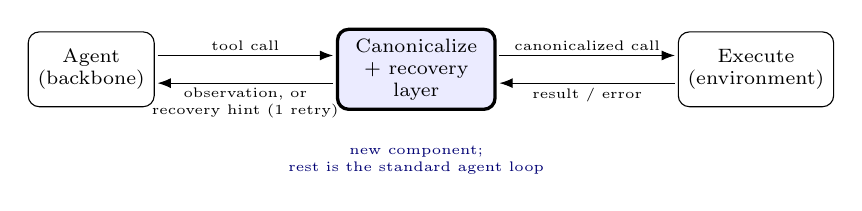
\begin{tikzpicture}[
  >=Latex,
  agent/.style={draw, rounded corners, align=center, minimum height=0.95cm, minimum width=1.6cm, font=\scriptsize},
  layer/.style={draw, very thick, rounded corners, fill=blue!8, align=center, minimum height=0.95cm, minimum width=2.0cm, font=\scriptsize},
  env/.style={draw, rounded corners, align=center, minimum height=0.95cm, minimum width=1.6cm, font=\scriptsize},
  fwd/.style={->, shorten >=1pt, shorten <=1pt},
  lbl/.style={font=\tiny, inner sep=1.5pt}
]
\node[agent] (a) {Agent\\(backbone)};
\node[layer, right=2.3cm of a] (L) {Canonicalize\\$+$ recovery\\layer};
\node[env, right=2.3cm of L] (e) {Execute\\(environment)};
% outgoing (top): agent -> layer -> env
\draw[fwd] ([yshift=5pt]a.east) -- node[lbl, above] {tool call} ([yshift=5pt]L.west);
\draw[fwd] ([yshift=5pt]L.east) -- node[lbl, above] {canonicalized call} ([yshift=5pt]e.west);
% returning (bottom): env -> layer -> agent
\draw[fwd] ([yshift=-5pt]e.west) -- node[lbl, below] {result / error} ([yshift=-5pt]L.east);
\draw[fwd] ([yshift=-5pt]L.west) -- node[lbl, below, align=center] {observation, or\\ recovery hint ($1$ retry)} ([yshift=-5pt]a.east);
\node[font=\tiny, align=center, below=0.32cm of L, text=blue!45!black] {new component;\\ rest is the standard agent loop};
\end{tikzpicture}}
\captionof{figure}{The canonicalization-plus-recovery layer (blue, the only new
component) sits between the agent and the environment and mediates both
directions. Outgoing tool calls have their argument values canonicalized to the
schema's language and format before execution; on an execution error the layer
returns a structured English recovery hint and allows one retry, otherwise it
passes the observation back unchanged. It is model-agnostic and adds no
parameters.}
\label{fig:pipeline}

\end{center}

\end{document}
